\documentclass[border=10pt]{standalone}
\usepackage{tikz}

\tikzstyle{vertex}=[circle,draw,fill=black!20,minimum size=0.7cm,inner sep=0pt]
\tikzstyle{edge} = [draw,thick,-]
\tikzstyle{weight} = [font=\small,sloped]

\begin{document}
\noindent
    \centering
    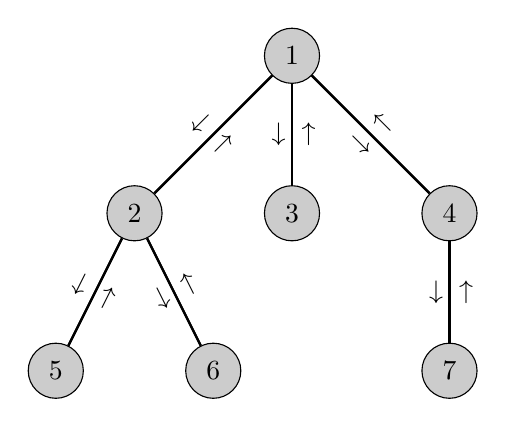
\begin{tikzpicture}[scale=1.0,transform shape,auto,swap]
        \node[vertex] (1) at (0, 0) {1};
        \node[vertex] (2) at (-2, -2) {2};
        \node[vertex] (3) at (0, -2) {3};
        \node[vertex] (4) at (2, -2) {4};
        \node[vertex] (5) at (-3, -4) {5};
        \node[vertex] (6) at (-1, -4) {6};
        \node[vertex] (7) at (2, -4) {7};
        \path[edge] (1) -- node[weight,above] {$\leftarrow$} (2);
        \path[edge] (1) -- node[weight,above] {$\leftarrow$} (3);
        \path[edge] (1) -- node[weight,above] {$\leftarrow$} (4);
        \path[edge] (2) -- node[weight,above] {$\leftarrow$} (5);
        \path[edge] (2) -- node[weight,above] {$\leftarrow$} (6);
        \path[edge] (4) -- node[weight,above] {$\leftarrow$} (7);
        \path[edge] (1) -- node[weight,below] {$\rightarrow$} (2);
        \path[edge] (1) -- node[weight,below] {$\rightarrow$} (3);
        \path[edge] (1) -- node[weight,below] {$\rightarrow$} (4);
        \path[edge] (2) -- node[weight,below] {$\rightarrow$} (5);
        \path[edge] (2) -- node[weight,below] {$\rightarrow$} (6);
        \path[edge] (4) -- node[weight,below] {$\rightarrow$} (7);
    \end{tikzpicture}
\end{document}
